\usetikzlibrary{calc,arrows.meta,positioning,backgrounds}
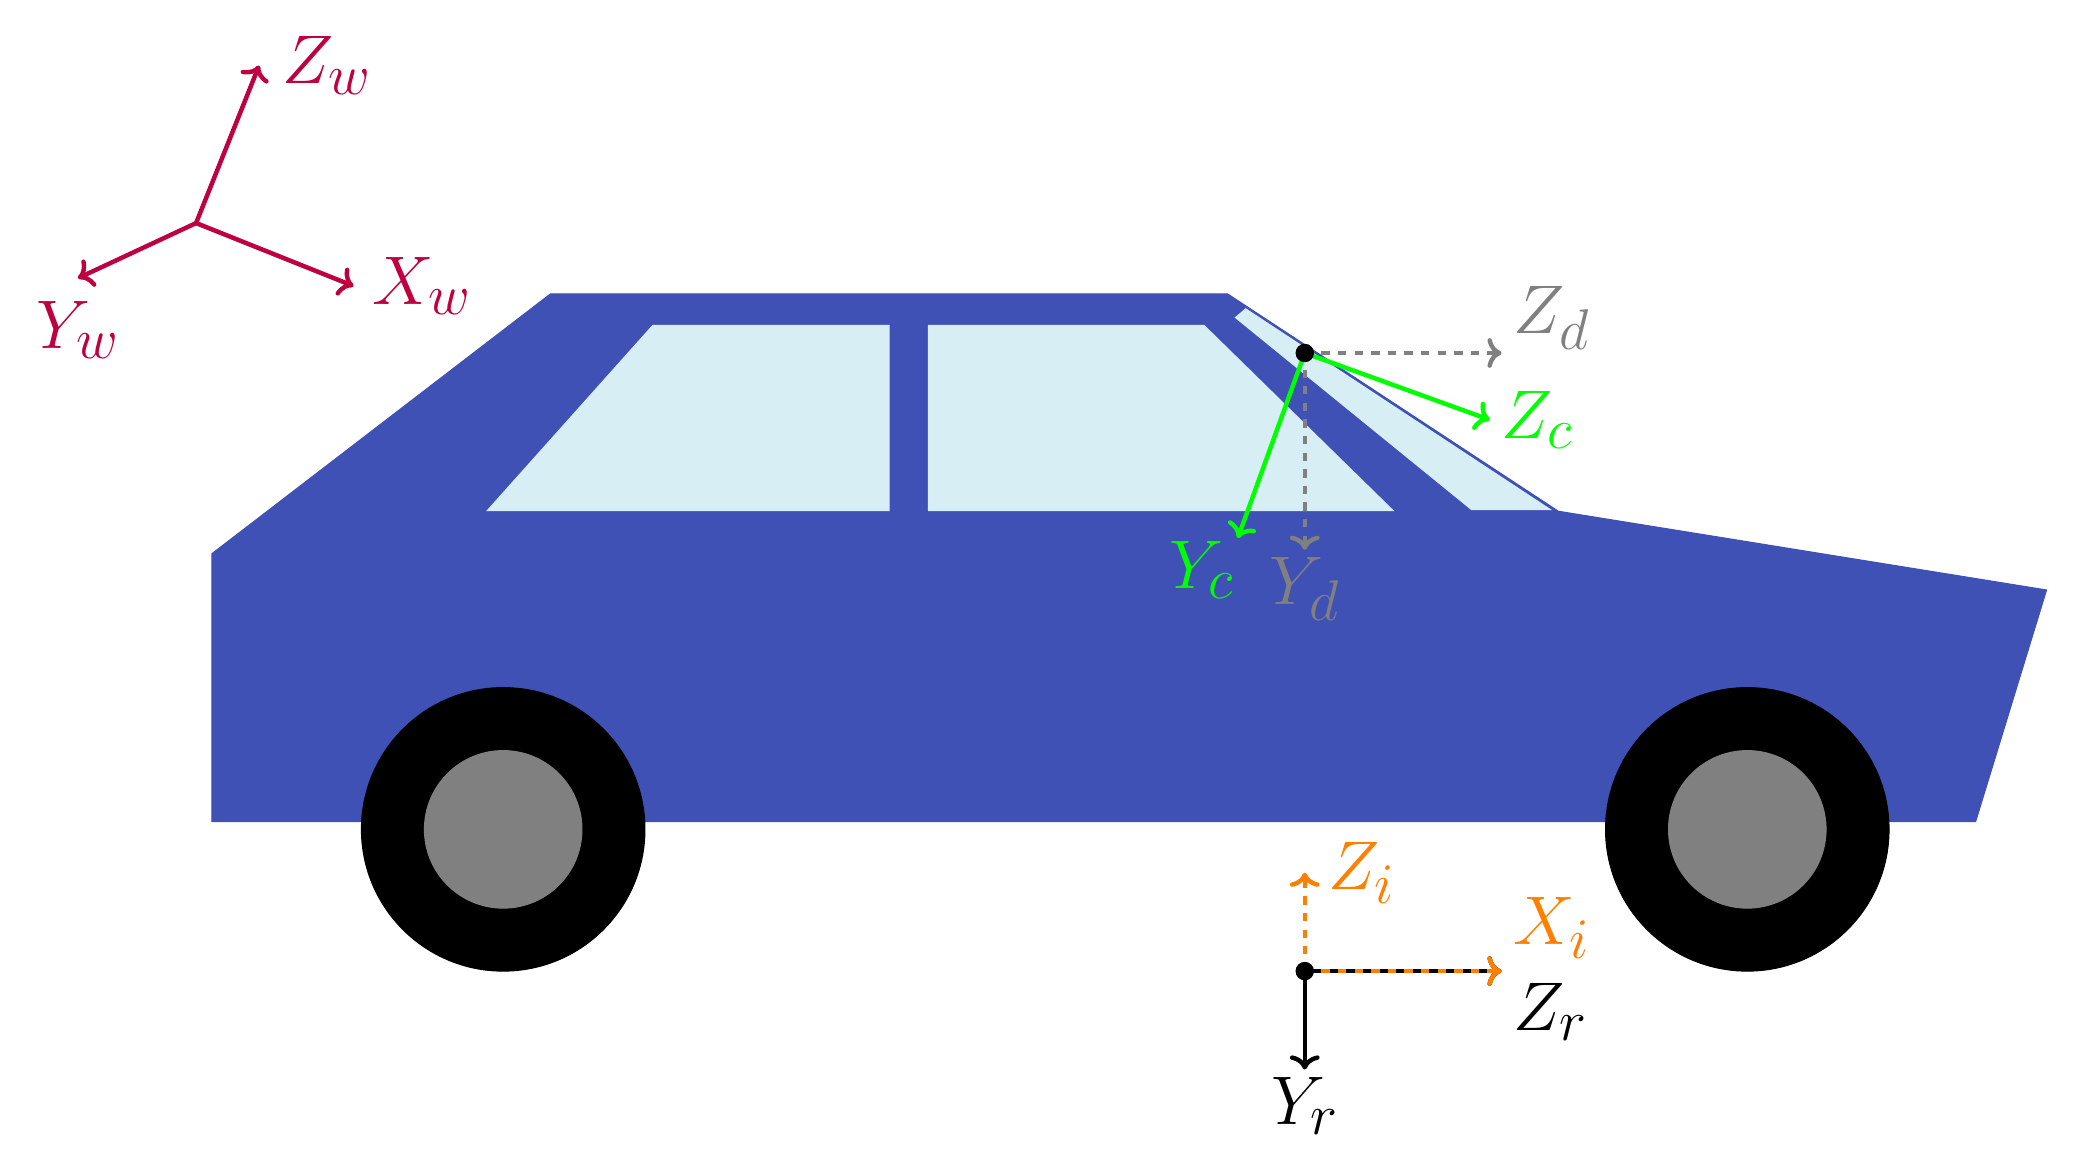
\begin{tikzpicture} [
    description/.style={draw=gray!70, thick, line cap=round, every node/.style={align=center, font=\scriptsize\sffamily, anchor=north}},
imagearrow/.style={red, line cap=round, -{Triangle[width=3*#1]}, line width=#1, shorten >=#1*0*1.75pt, every node/.append style={fill, circle, inner sep=0pt, minimum size=#1*3.5pt, anchor=center, outer sep=0pt}}
  ]

\definecolor{bluewindow}{RGB}{215,238,244}
\definecolor{bluecar}{RGB}{64,81,181}


%\node[inner sep=0pt] (russell) at (0,0)
 %   {\includegraphics{Capture.png}};


\draw[color=bluecar, fill] (-11.3,0.2) -- (-7,3.5) -- (1.6,3.5) -- (5.8,0.74) -- (12,-0.26) -- (11.1, -3.2) -- (-11.3, -3.2) -- cycle;
\draw[color=bluewindow, fill] (-2.2,3.1) -- (1.3,3.1) -- (3.7,0.75) -- (-2.2,0.75) -- cycle;
\draw[color=bluewindow, fill](1.83,3.31) -- (1.7,3.2) -- (4.7,0.76) -- (5.7,0.76) -- cycle;
\draw[color=bluewindow,fill] (-5.7,3.1) -- (-2.7,3.1) -- (-2.7,0.75) -- (-7.8,0.75) -- cycle;

\draw[fill] (-7.6,-3.3) circle(1.8);
\draw[fill, gray] (-7.6,-3.3) circle(1);

\draw[fill] (8.2,-3.3) circle(1.8);
\draw[fill, gray] (8.2,-3.3) circle(1);


% coordinate systems
%\draw [<->,ultra thick, dashed] (3,4.3) node (yaxis) [right] {\LARGE $X_c$}
 %       |- (5,2.7) node (xaxis) [below] {\LARGE $Z_c$};

% define some math for coordinate axes
\pgfmathsetmacro{\len}{2.5}
\pgfmathsetmacro{\cosp}{0.94}
\pgfmathsetmacro{\sinp}{0.34}

\pgfmathsetmacro{\ocx}{2.58}
\pgfmathsetmacro{\ocy}{2.75}

\pgfmathsetmacro{\orx}{2.58}
\pgfmathsetmacro{\ory}{-5.1}

\pgfmathsetmacro{\owx}{-11.5}
\pgfmathsetmacro{\owy}{4.4}
\pgfmathsetmacro{\eps}{0.8}

% cam system
\draw[->, ultra thick, green] (\ocx,\ocy) -- (\ocx-\len*\sinp, \ocy-\len*\cosp) node[below left=-0.1 and -0.1]{\Huge $Y_c$};
\draw[->, ultra thick, green] (\ocx,\ocy) -- (\ocx+\len*\cosp, \ocy-\len*\sinp) node[right]{\Huge $Z_c$};

%default system
\draw[->, ultra thick, dashed, gray] (\ocx,\ocy) -- (\ocx, \ocy-\len) node[below=-0.05]{\Huge $Y_d$};
\draw[->, ultra thick, dashed, gray] (\ocx,\ocy) -- (\ocx+\len, \ocy) node[above right= -0.1 and 0]{\Huge $Z_d$};

%road system
\draw[->, ultra thick] (\orx,\ory) -- (\orx, \ory-\len*0.5) node[below=-0.05]{\Huge $Y_r$};
\draw[->, ultra thick] (\orx,\ory) -- (\orx+\len, \ory) node[below right= 0.01 and 0]{\Huge $Z_r$};

% road system ISO 8855
\draw[->, ultra thick, dashed, orange] (\orx,\ory) -- (\orx, \ory+0.5*\len) node[right=0.15]{\Huge $Z_i$};
\draw[->, ultra thick, dashed, orange] (\orx,\ory) -- (\orx+\len, \ory) node[above right= 0.01 and 0]{\Huge $X_i$};

% world
\draw[->, ultra thick, purple] (\owx, \owy) -- (\owx+\eps, \owy+2) node[right=0.15]{\Huge $Z_w$};
\draw[->, ultra thick, purple] (\owx, \owy) -- (\owx+2, \owy-\eps) node[right=0.1]{\Huge $X_w$};
\draw[->, ultra thick, purple] (\owx, \owy) -- (\owx-1.5, \owy - 1.5+\eps) node[below=0.15]{\Huge $Y_w$};


\draw[fill] (\ocx,\ocy) circle(0.11);
\draw[fill] (\orx,\ory) circle(0.11);

\end{tikzpicture}